\documentclass[letterpaper, 10 pt, conference]{ieeeconf}  % Comment this line out if you need a4paper
%\documentclass[a4paper, 10pt, conference]{ieeeconf}   % Use this line for a4 paper
\IEEEoverridecommandlockouts                                    % This command is only needed if you want to use the \thanks command
\overrideIEEEmargins                                                 % Needed to meet printer requirements.

%In case you encounter the following error:
%Error 1010 The PDF file may be corrupt (unable to open PDF file) OR
%Error 1000 An error occurred while parsing a contents stream. Unable to analyze the PDF file.
%This is a known problem with pdfLaTeX conversion filter. The file cannot be opened with acrobat reader
%Please use one of the alternatives below to circumvent this error by uncommenting one or the other
%\pdfobjcompresslevel=0
%\pdfminorversion=4

% See the \addtolength command later in the file to balance the column lengths
% on the last page of the document

\usepackage{graphicx}    % for pdf, bitmapped graphics files
%\usepackage{epsfig}    % for postscript graphics files
\usepackage{mathptmx} % assumes new font selection scheme installed
\usepackage{times}        % assumes new font selection scheme installed
\usepackage{amsmath}  % assumes amsmath package installed
\usepackage{amssymb}  % assumes amsmath package installed
\usepackage{listings}

\title{\LARGE \bf Formation Control}

\author{Ajay Ahir, Ben Philps and Sumaiyah Kola}

\begin{document}

\maketitle
\thispagestyle{empty}
\pagestyle{empty}

%%%%%%%%%%%%%%%%%%%%%%%%%%%%%%%%%%%%%%%%%%%%%%%%%%%%%%%%%%%%%%%%%%%%%%%%%%%%%%%%
\begin{abstract}

Multi-robot teams may need to move in formation for various reasons such as surveillance or for display. This report describes a project undertaken to perform the navigation of multi-robot teams with formation control using a behavior based approach. Behaviors generate velocities that combine to lead each robot, such as by generating a velocity to avoid obstacles and a velocity to remain in formation. These behaviors are extended to switch formation in tight gaps such as corridors. Both a centralized and decentralized solution are shown.

\end{abstract}


%%%%%%%%%%%%%%%%%%%%%%%%%%%%%%%%%%%%%%%%%%%%%%%%%%%%%%%%%%%%%%%%%%%%%%%%%%%%%%%%
\section{INTRODUCTION}

In application domains such as exploration, surveillance and 'search and rescue', coordination and control mechanisms for multiple robots have been shown to provide cost effective and fault tolerant solutions \cite{c1}.

Inspired by the natural coordinated behaviour of bird flocking and ant swarming, formation control of multiple robots can improve surveillance coverage by combining sensor readings from individual agents. The main objective is for multiple robots to traverse the environment while maintaining an explicitly specified spacing relationship between agents.

In this paper we provide a centralised behaviour-based approach to formation control. This solution relies on each agent transmitting and receiving information from a global controller. We also provide a robust and fault-tolerant decentralised approach suitable when communication is restricted.

\section{BACKGROUND}
Balch and Arkin provide a behaviour-based approach to formation control, splitting the task into behavioural components, referred to as 'motor schemas' \cite{c2}. 

\subsection{Motor Schemas}

Each motor schema generates a vector (direction and magnitude of movement) given the current sensor inputs and positions of other robots. Motor schemas, goal-navigation, static/dynamic obstacle avoidance and formation-maintenance generate vectors, $\vec{V}_{goal}, \vec{V}_{static\_obs}, \vec{V}_{dynamic\_obs}, \vec{V}_{form}$ respectively. A gain value, $g$, dictates the contribution of each schema to the overall behaviour. 

The overall behavioural response, $\vec{V}$, is calculated by weighting each vector by its gain value and summing and normalising the results. To overcome local minima and maxima, an additional schema generating noise, $\vec{V}_{noise}$, is included.

\subsection{Formation Maintenance}

To compute $\vec{V}_{form}$ for robot $R_i$ in position $P_{R_i}$,
\[\vec{V}_{form} = P_{desired} - P_{R_i}\]
where $P_{desired}$ is the desired position of $R_i$ in the formation.

TODO: where $P_{desired}$ comes from...

The magnitude of $\vec{V}_{form}$ depends on the distance from $P_{R_i}$ to $P_{desired}$. 'Zones' are defined around $P_{desired}$ as seen in figure \ref{formation_zones}. 

Within the \textit{dead zone}, the robot is considered in formation and so $\vec{V}_{form} = \vec{0}$. Within the \textit{control zone}, the magnitude linearly increases from the inner edge. The magnitude at the outer edge of the \textit{control zone} is propagated throughout the \textit{ballistic zone}.

\begin{figure}[ht]
\centering
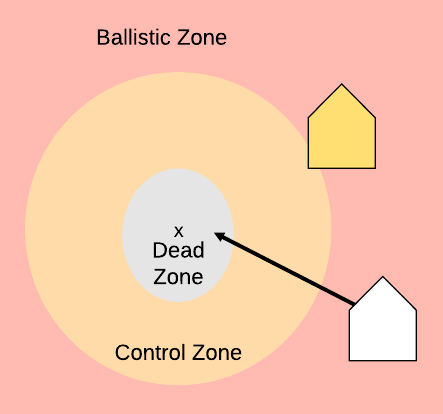
\includegraphics[width=0.45\linewidth]{images/formation_zones.png}
\caption{Zones for computing $\vec{V}_{form}$ with $P_{desired}$ marked as 'x'}
\label{formation_zones}
\end{figure}

We implement a leader-reference behaviour-based approach to formation control, extending the work of \cite{c2} to incorporate a formation switching strategy.

\section{EXPERIMENTAL SET-UP}

We conduct experiments on TurtleBot3 \cite{turtlebot} robots controlled using ROS \cite{ros} with Gazebo \cite{gazebo} as the simulation environment. We assume all robots are identical and labelled 
with $R_0$ designated leader and $R_1,...R_n$ followers. Here $n$ is 5.

Our evaluation considers the performance of robot formations in multiple arenas that include obstacles, narrow corridors and tight corners. Figure \ref{corridorworld} illustrates one of the testing arenas.

\begin{figure}[thpb]
\centering
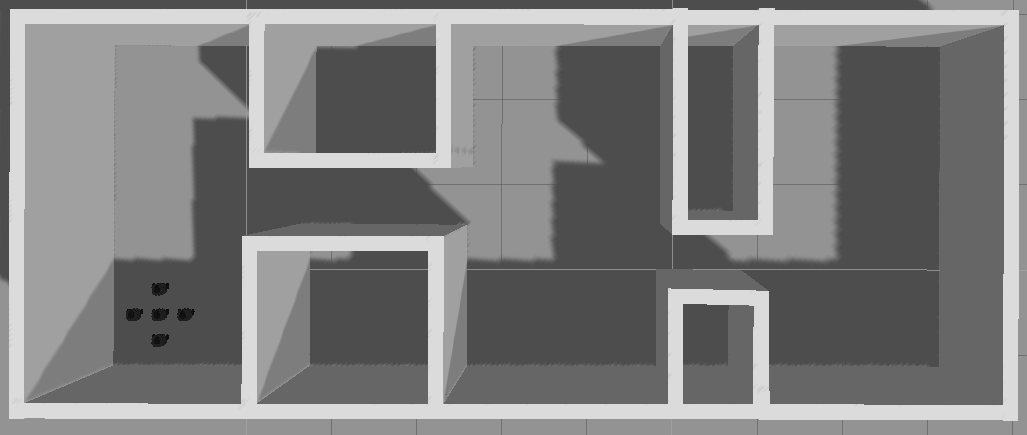
\includegraphics[width=\linewidth]{images/corridorworld.png}
\caption{The \textit{diamond} formation in an arena with tight corridors}
\label{corridorworld}
\end{figure}

\section{APPROACH}
\subsection{Formations}
In our implementation \cite{repository}, several formations for five robots are considered: \textit{diamond}, \textit{column}, \textit{line} and \textit{wedge} (figure \ref{formation_shapes}). The spacing of the robots in the formation can be altered. 
   
\begin{figure}[thpb]
\centering
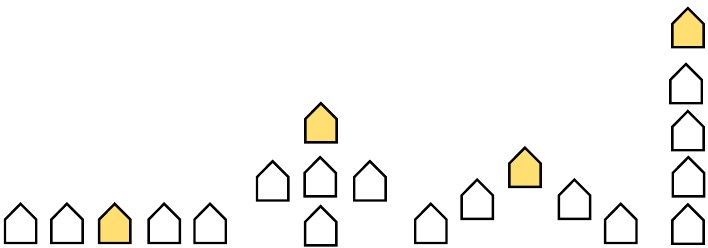
\includegraphics[width=0.7\linewidth]{images/formation_shapes.jpg}
\caption{Formations L-R: \textit{line}, \textit{diamond}, \textit{wedge}, \textit{column} with leader coloured}
\label{formation_shapes}
\end{figure}

\subsection{Motor Schemas}
The behaviour response, $\vec{V}$, for each robot is calculated,
\begin{equation*}
\begin{aligned}
\vec{V} =   & g_{goal} \vec{V}_{goal} + g_{obs} \vec{V}_{ob} + \vec{V}_{noise}        && \text{if leader}\\
      & g_{form} \vec{V}_{form} + g_{obs} \vec{V}_{obs} + \vec{V}_{noise}       && \text{if follower}\\
\end{aligned}
\end{equation*}
where vector $\vec{V}_{noise}$ has a magnitude of 0.2. 
TODO: explain why the formulas are like above \\
TODO: put how $\vec{V}_{goal}$ is normalised and $\vec{V}_{obs}$ and $\vec{V}_{formation}$ are scaled to be in $[0,1]$

\begin{table}[h]
\label{table_example}
\begin{center}
\begin{tabular}{|c||c||c c|}
\hline
Motor Schema & Gain Value)\\
\hline
Goal Navigation             & 0.8 \\
Static Obstacle Avoidance   & 1.0 \\
Formation Maintenance       & 0.9 \\
\hline
\end{tabular}
\end{center}
\caption{Motor Schema Gain Values, $g$}
\end{table}

TODO: Feedback linearisation with $\epsilon$ of 0.2m.

Motor schemas for goal navigation, obstacle avoidance and formation maintenance are defined below.

\subsubsection*{Goal Navigation}
$\vec{V}_{goal}$ points from the leader, $R_0$, to the next point along a path from $R_0$ to the goal. A path is generated using an optimised version of the rapidly-exploring random trees (RRT) algorithm, RRT*. RRT efficiently explores the search space by building a space-filling tree. Additional rewiring and cost minimisation steps can generate an approximate shortest path to the goal. The magnitude of $\vec{V}_{goal}$ is 1.

\subsubsection*{Static Obstacle Avoidance}
\subsubsection*{Dynamic Obstacle Avoidance}
\subsubsection*{Formation Maintenance}
\begin{table}[h]
\label{table_formation}
\begin{center}
\begin{tabular}{|c || c||c |}
\hline
 & Parameter & Value (m)\\
\hline
(1) & Spacing Distance            & 0.8 \\
(2) & Dead Zone Radius            & $1.5 \times radius(robot)$\\
(3) & Control Zone Radius         & (2) $+$ (3) \\
\hline
\end{tabular}
\end{center}
\caption{Formation Maintenance Parameters}
\end{table}

\subsection{Formation Switching Strategy}
\subsection{Decentralised}
The centralised algorithm relies on knowledge of all robot positions as well as their combined view of the world. Our decentralised solution achieves this with limited message passing between robots to communicate the required state. Communication links are defined between certain robots in each formation. For \textit{line}, \textit{column} and \textit{wedge}, links are defined between adjacent robots. For \textit{diamond}, all robots are arranged so they can communicate with the center robot.  
//
TODO: talk abou diff arenas \\
TODO: talk about how we test things

\section{results}

\section{conclusion}




\addtolength{\textheight}{-12cm}   % This command serves to balance the column lengths
                                  % on the last page of the document manually. It shortens
                                  % the textheight of the last page by a suitable amount.
                                  % This command does not take effect until the next page
                                  % so it should come on the page before the last. Make
                                  % sure that you do not shorten the textheight too much.

%%%%%%%%%%%%%%%%%%%%%%%%%%%%%%%%%%%%%%%%%%%%%%%%%%%%%%%%%%%%%%%%%%%%%%%%%%%%%%%%
\section{ACKNOWLEDGMENT}

\begin{itemize}
\item Ajay Ahir - Worked on setting up the multi-robot environment and obstacle avoidance. Added the RRT* component and worked on combining velocities. Decentralized the solution and produced the error plots.
\item Ben Philps - 
\item Sumaiyah Kola - 
\end{itemize}

%%%%%%%%%%%%%%%%%%%%%%%%%%%%%%%%%%%%%%%%%%%%%%%%%%%%%%%%%%%%%%%%%%%%%%%%%%%%%%%%

Appendixes should appear before the acknowledgment.

\begin{thebibliography}{99}

\bibitem{c1} J. S. Jennings, G. Whelan and W. F. Evans, "Cooperative search and rescue with a team of mobile robots," 1997 8th International Conference on Advanced Robotics. Proceedings. ICAR'97, Monterey, CA, USA, 1997, pp. 193-200.
\bibitem{c2} T. Balch and R. C. Arkin, "Behavior-based formation control for multirobot teams," in IEEE Transactions on Robotics and Automation, vol. 14, no. 6, pp. 926-939, Dec. 1998.
\bibitem{gazebo} Gazebo. http://gazebosim.org/
\bibitem{ros} ROS - Robot Operating System. https://www.ros.org/
\bibitem{turtlebot} Turtlebot3. http://emanual.robotis.com/docs/en/platform/turtlebot3/overview/
\bibitem{repository} Code Repository. https://github.com/DoodleBobBuffPants/RobotProject
%%%%%%%%%%%%%%%%%%%%%%%%%%%

\end{thebibliography}




\end{document}
